\documentclass[12pt,titlepage]{article}
\usepackage[margin=1.25in]{geometry}
\usepackage{graphicx,amsmath,enumitem}

%% Variables definition
\newcommand{\vSubject}{Matematika 3}
\newcommand{\vSubtitle}{Graph Theory}
\newcommand{\vName}{Dicha Zelianivan Arkana}
\newcommand{\vNIM}{2241720002}
\newcommand{\vClass}{2i}
\newcommand{\vDepartment}{Information Technology}
\newcommand{\vStudyProgram}{D4 Informatics Engineering}

%% [START] Tikz related stuff
\usepackage{tikz}
\usetikzlibrary{svg.path,calc,shapes.geometric,shapes.misc}
\tikzstyle{terminator} = [rectangle, draw, text centered, rounded corners = 1em, minimum height=2em]
\tikzstyle{preparation} = [chamfered rectangle, chamfered rectangle sep=0.75em, draw, text centered, minimum height = 2em]
\tikzstyle{process} = [rectangle, draw, text centered, minimum height=2em]
\tikzstyle{decision} = [diamond, aspect=2, draw, text centered, minimum height=2em]
\tikzstyle{data}=[trapezium, draw, text centered, trapezium left angle=60, trapezium right angle=120, minimum height=2em]
\tikzstyle{connector} = [line width=0.25mm]
%% [END] Tikz related stuff

%% [START] Fancy header related stuff
\usepackage{fancyhdr}
\pagestyle{fancy}
\setlength{\headheight}{15pt} % compensate fancyhdr style
\fancyhead{}
\fancyfoot{}
\fancyfoot[L]{\thepage}
\fancyfoot[R]{\textit{\vSubject - \vSubtitle}}
\renewcommand{\footrulewidth}{0.4pt}% default is 0pt, overline for footer
%% [END] Fancy header related stuff

%% [START] Custom tabular command related stuff
\usepackage{tabularx}
\newcommand{\details}[2]{
    #1 & #2  \\
}
%% [END] Custom tabular command related stuff

%% [START] Figure related stuff
\newcommand{\image}[3][1]{
    \begin{figure}[h]
        \centering
        \includegraphics[#1]{#2}
        \caption{#3}
        \label{#3}
    \end{figure}
}
%% [END] Figure related stuff

\begin{document}
\begin{titlepage}
    \centering
    \vfill
    {\bfseries\LARGE
        \vSubject\\
        \vskip0.25cm
        \vSubtitle
    }
    \vfill
    
\includegraphics[width=6cm]{images/polinema-logo.png}
    \vfill
    {
        \textbf{Name}\\
        \vName\\
        \vskip0.5cm
        \textbf{NIM}\\
        \vNIM\\
        \vskip0.5cm
        \textbf{Class}\\
        \vClass\\
        \vskip0.5cm
        \textbf{Department}\\
        \vDepartment\\
        \vskip0.5cm
        \textbf{Study Program}\\
        \vStudyProgram
    }
\end{titlepage}

\tableofcontents

\pagebreak

\section{Question 1}
\begin{enumerate}[label=\alph*.)]
    \item {
        Tuliskan himpunan simpul / vertex (V) dan sisi / edge (E) dari graf di bawah ini!
        \begin{center}
            \includegraphics*[height=4cm]{./images/graph-1.png}
        \end{center}

        \begin{itemize}
            \item {
                Himpunan simpul / vertex (V)
                \begin{equation*}
                    V = \{1, 2, 3, 4\}
                \end{equation*}
            }
            \item {
                Himpunan sisi / edge (E)
                \begin{align*}
                    E &= \{e1, e2, e3, e4, e5, e6, e7, e8\}\\
                    E &= \{(1,2), (2,3), (1,3), (1,3), (2,4), (3,4), (3,4), (3,3))\}
                \end{align*}
            }
        \end{itemize}
    }
    \item {
        Pada gambar tersebut, sebutkan simpul-simpul yang bertetangga dengan simpul 1, 2, 3, dan 4!
        \begin{itemize}
            \item \textbf{Simpul 1 :} 2, 3
            \item \textbf{Simpul 2 :} 1, 3, 4
            \item \textbf{Simpul 3 :} 1, 2, 4
            \item \textbf{Simpul 4 :} 2, 3
        \end{itemize}
    }
    \item {
        Sebutkan sisi-sisi yang bersisian dengan simpul 1, 2, 3, dan 4!
        \begin{itemize}
            \item \textbf{Simpul 1 :} e1, e3, e4
            \item \textbf{Simpul 2 :} e1, e2, e5
            \item \textbf{Simpul 3 :} e2, e3, e4, e6, e7, e8
            \item \textbf{Simpul 4 :} e5, e6, e7
        \end{itemize}
    }
    \item {
        Berapa derajat dari simpul 1, 2, 3, dan 4?

        \begin{itemize}
            \item \textbf{Simpul 1 :} 3
            \item \textbf{Simpul 2 :} 3
            \item \textbf{Simpul 3 :} 6
            \item \textbf{Simpul 4 :} 3
        \end{itemize}
    }
    \item {
        Sebutkan 6 buah lintasan yang ada pada graf tersebut!

        \begin{itemize}
            \item \textbf{Lintasan 1 :} $1 \rightarrow e1 \rightarrow 2 \rightarrow e5 \rightarrow 4$
            \item \textbf{Lintasan 2 :} $1 \rightarrow e3 \rightarrow 3 \rightarrow e6 \rightarrow 4$
            \item \textbf{Lintasan 3 :} $1 \rightarrow e4 \rightarrow 3 \rightarrow e7 \rightarrow 4$
            \item \textbf{Lintasan 4 :} $2 \rightarrow e2 \rightarrow 3 \rightarrow e6 \rightarrow 4$
            \item \textbf{Lintasan 5 :} $2 \rightarrow e5 \rightarrow 4$
        \end{itemize}
    }
\end{enumerate}

\section{Question 2}
Berilah contoh graf tidak kosong paling sederhana yang memenuhi kondisi berikut:
\begin{enumerate}[label=\alph*.)]
    \item {
        Tidak memiliki simpul berderajat ganjil

        \begin{center}
            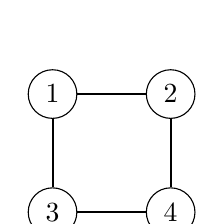
\begin{tikzpicture}[node distance=1.5cm]
                \node (1) [circle, draw] {1};
                \node (2) [circle, draw, right of=1] {2};
                \node (3) [circle, draw, below of=1] {3};
                \node (4) [circle, draw, right of=3] {4};

                \draw [connector] (1) -- (2);
                \draw [connector] (1) -- (3);
                \draw [connector] (2) -- (4);
                \draw [connector] (3) -- (4);
            \end{tikzpicture}
        \end{center}
    }
    \item {
        Tidak memiliki titik berderajat genap

        \begin{center}
            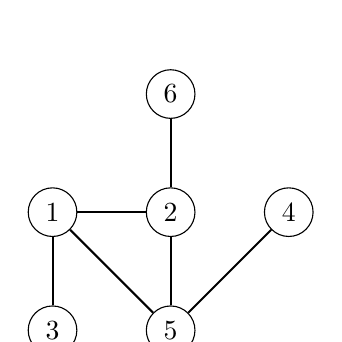
\begin{tikzpicture}[node distance=1.5cm]
                \node (1) [circle, draw] {1};
                \node (2) [circle, draw, right of=1] {2};
                \node (3) [circle, draw, below of=1] {3};
                \node (4) [circle, draw, right of=2] {4};
                \node (5) [circle, draw, below of=2] {5};
                \node (6) [circle, draw, above of=2] {6};

                \draw [connector] (1) -- (2);
                \draw [connector] (1) -- (3);
                \draw [connector] (1) -- (5);
                \draw [connector] (4) -- (5);
                \draw [connector] (2) -- (5);
                \draw [connector] (2) -- (6);
            \end{tikzpicture}
        \end{center}
    }
    \item {
        Memiliki tepat 1 titik berderajat ganjil

        It's not possible since it would violate the Handshaking Lemma.
    }
    \item {
        Memiliki tepat 2 titik berderajat ganjil

        \begin{center}
            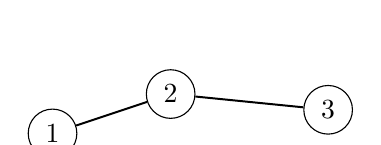
\begin{tikzpicture}[node distance=1.5cm]
                \node (1) [circle, draw] {1};
                \node (2) [circle, draw, right of=1, yshift=5mm] {2};
                \node (3) [circle, draw, right of=2, xshift=5mm, yshift=-2mm] {3};

                \draw [connector] (1) -- (2);
                \draw [connector] (2) -- (3);
            \end{tikzpicture}
        \end{center}
    }
\end{enumerate}

\section{Question 3}
Tentukan apakah ada graf sederhana dengan 5 titik yang masing-masing berderajat
berikut ini. Jika ada, gambarkan graf tersebut!
\begin{enumerate}[label=\alph*.)]
    \item {
        3, 3, 3, 2, 3

        \begin{center}
            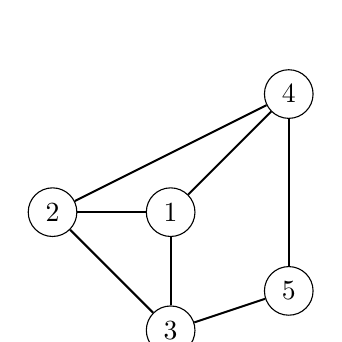
\begin{tikzpicture}[node distance=1.5cm]
                \node (1) [circle, draw] {1};
                \node (2) [circle, draw, left of=1] {2};
                \node (3) [circle, draw, below of=1] {3};
                \node (4) [circle, draw, right of=1, yshift=1.5cm] {4};
                \node (5) [circle, draw, right of=1, yshift=-1cm] {5};

                \draw [connector] (1) -- (2);
                \draw [connector] (1) -- (3);
                \draw [connector] (1) -- (4);
                \draw [connector] (2) -- (3);
                \draw [connector] (2) -- (4);
                \draw [connector] (4) -- (5);
                \draw [connector] (3) -- (5);
            \end{tikzpicture}
        \end{center}
    }
    \item {
        1, 2, 4, 3, 5

        This is not possible since it would violate the Handshaking Lemma.
        The odd degree must be even, in this case there are 3 of them which are 1, 3, and 5.
    }
    \item {
        1, 2, 3, 4, 4

        \begin{center}
            \includegraphics*[height=4cm]{./images/graph-3c.png}
        \end{center}
    }
    \item {
        0, 1, 2, 2, 3

        \begin{center}
            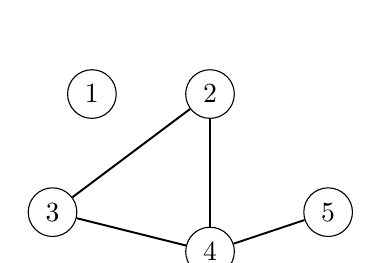
\begin{tikzpicture}[node distance=1.5cm]
                \node (1) [circle, draw] {1};
                \node (2) [circle, draw, right of=1] {2};
                \node (3) [circle, draw, below of=1, xshift=-5mm] {3};
                \node (4) [circle, draw, below of=2, yshift=-5mm] {4};
                \node (5) [circle, draw, right of=4, yshift=5mm] {5};

                \draw [connector] (2) -- (4);
                \draw [connector] (2) -- (3);
                \draw [connector] (3) -- (4);
                \draw [connector] (5) -- (4);
            \end{tikzpicture}
        \end{center}
    }
\end{enumerate}

\pagebreak

\section{Question 4}
Carilah 3 contoh penerapan graph dalam kehidupan sehari-hari

\begin{enumerate}
    \item {
        Graph in Social Media connection. It's being used to determine the
        connection between users in social media. It's also being used to
        determine the connection between users and the content they like.
        This can be used to determine the content that the user might like
        or users they might know.
    }
    \item {
        Graph in Google Maps. It's being used to determine the distance
        between two places. It's also being used to determine the shortest
        path between two places. More specifically the one being used is usually a
        weighted graph.
    }
    \item {
        Graph in Computer Network Topology. It's being used to determine the
        connection between computers. It's also being used to determine the
        nearest computer to a computer. This can be used to determine the
        shortest path between two computers which can determine the fastest
        way to send data between two computers.
    }
\end{enumerate}

\end{document}

